% Basic US Letter document format
% by C. G. Wilson 
% modified by Morgan Fine-Morris

\documentclass[11pt]{article}
\usepackage{amsfonts}
\usepackage[pdftex]{graphicx}
\usepackage[space]{grffile}
\usepackage{caption}
\usepackage{subcaption}
\usepackage{placeins}

% \usepackage{palatino}

%%formatting
\textwidth 6.85in
\textheight 8.75in

\pagestyle{headings}
%\markright{\today, header}

\newcommand{\tsscale}{0.45}
\newcommand{\bcscale}{0.3}


\begin{document}

%%formatting
\oddsidemargin -0.22in
\evensidemargin -0.22in
\topmargin 0.05in
\topskip 0.25in
\headheight 0.05in
\headsep 0.25in

\graphicspath{{"../Data and Analysis/long TB Yan/plots/"}{"../Data and Analysis/short TB Yan/plots/"}}
%{"../Data and Analysis/long TB Yan/plots/Comparative TS Yan/"}{"../Data and Analysis/long TB Yan/plots/Comparative TS TB/"}}
%\begin{center}
%\Large{\textbf{Results}}
%\end{center}


\FloatBarrier
\section{Results}
talk about time series - what features characterize each model?
-Compare models by comparing features of their time series: Burst Duration, Interburst Interval, etc. 
From these generally trend are clear: as
Simple visual comparison of a section of membrane potential time series reveals the general trends created
Yan model characterized by longer burst duration and more spiking along the leading edge of each burst.
Comparing time series Figures ~\ref{fig:ts18} and ~\ref{fig:ts42}, we see that at the low end of the tested $g_{NaP}$ range (1.8 nS)...and at the end of the range, when $g_{NaP}$ = 4.2 nS, we see ...


\begin{figure}[h]
	\centering
	\includegraphics[scale=\tsscale]{Comparative TS Yan/ts_gnaps1p8_eLall.pdf}
	\includegraphics[scale=\tsscale]{Comparative TS TB/ts_gnaps1p8_eLall.pdf}
	%\caption{Time series generated from Yan and TB models at all values of $eL$ for $g_{NaP}$ = 1.8 nS.}
	%\label{fig:ts18}
	\includegraphics[scale=\tsscale]{Comparative TS Yan/ts_gnaps4p2_eLall.pdf}
	\includegraphics[scale=\tsscale]{Comparative TS TB/ts_gnaps4p2_eLall.pdf}
	%\caption{Time series generated from Yan and TB models at all values of $eL$ for $g_{NaP}$ = 4.2 nS.}
	\label{fig:ts42}
\end{figure}

\subsection{Total Cycle Time, Burst Duration, Interburst Interval}


-Interesting to note that while most of the measures vary considerably depending on the model and parameters used to generate the time series, Total Cycle exhibits little-to-no change ~ref{fig:hm txt}. The single exception, caused by bi-modal bursting behavior ~\ref{fig:tsTb42}, occurs in the TB model when $eL$=-60.0 mV and $g_{NaP}$=4.2 nS. 

Average total cycle time, the time from the start of one burst to the start of another, was very uniform between models for all parameter sets that exhibited bursting (Fig [~\ref{fig:hm_tct}]). The only point of significant difference was at $eL=-60 g_{nap} = 4.2$ where the value for the TB model was half that of the Yan model, due to the two modes of interburst interval present in for the TB model but not for the Yan model (Fig [~\ref{fig:ts_6042}]).

\begin{figure}[h]
	\centering
	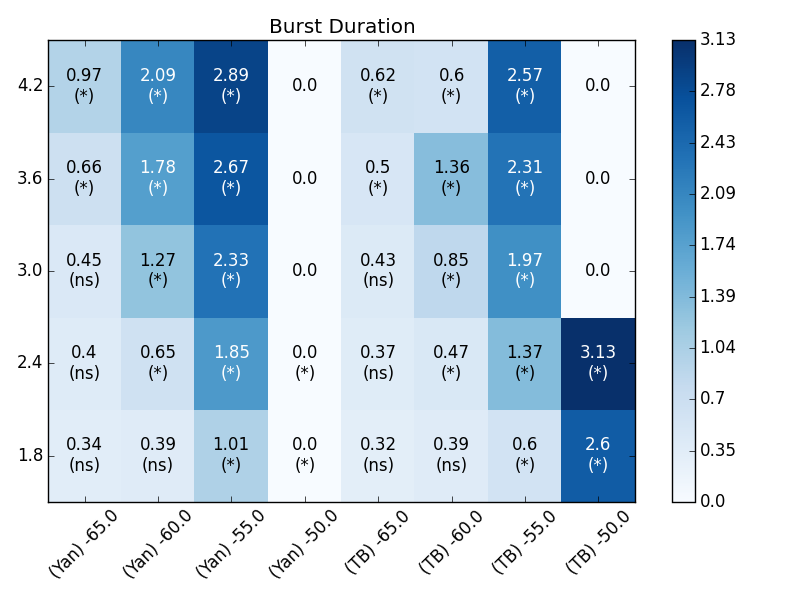
\includegraphics[scale=.4]{heatmap_Burst_Duration.png}
	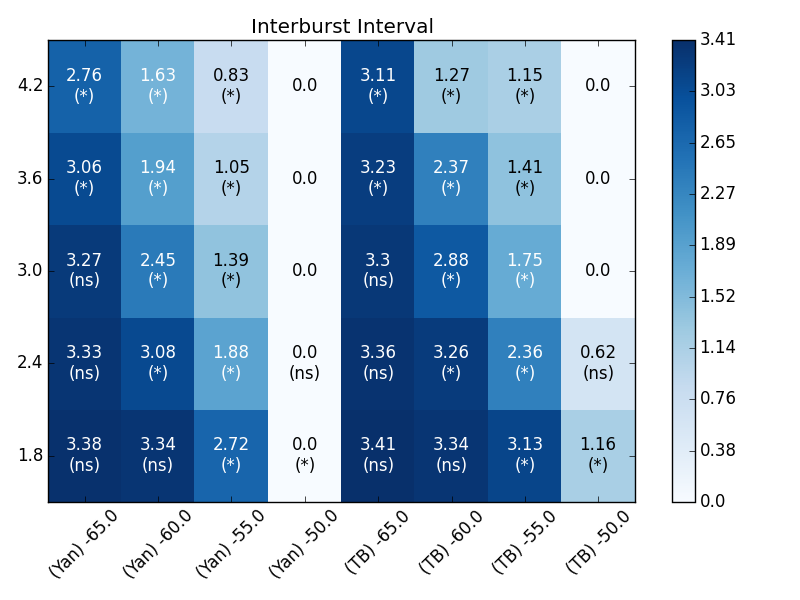
\includegraphics[scale=.4]{heatmap_Interburst_Interval.png}
	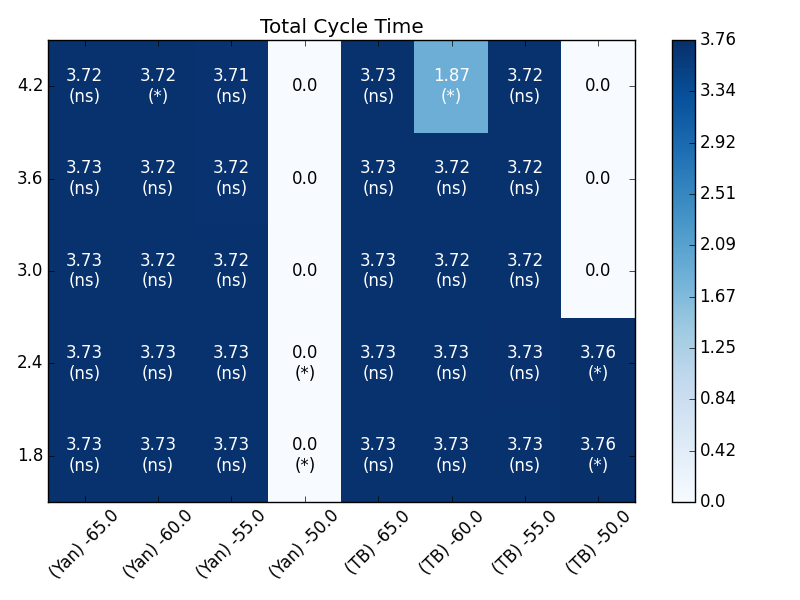
\includegraphics[scale=.4]{heatmap_Total_Cycle_Time.png}
	\caption{Heat map showing variations in total cycle time with changes in $eL$, $g_{NaP}$, and model. Zeroes indicate tonic spiking. Star (*) and (ns) symbols below each value indicates statistical significance between the corresponding cell for the other model.}
	\label{fig:hmTCT}
\end{figure}
 \begin{figure}[h]
	\centering
	\includegraphics[scale=\bcscale]{barchart_Burst_Duration.pdf}
	\includegraphics[scale=\bcscale]{barchart_Interburst_Interval.pdf}
	\caption{}
	\label{fig:bcBD}
\end{figure}
   


Where bursting occurs in the Yan model, burst duration for Yan increases more rapidly than TB as $eL$ increases. For $eL=-55 mV$, burst duration is different at all tested $g_{NaP}$ values.
Differences in burst duration between the two models does not change significantly with change in $g_{NaP}$. For Yan, bursting does not occur while $eL = -50 mV$, while bursting occurs at $eL=-50,\  g_{NaP}=1.8, 2.4$. 

With one exception, interburst interval and burst duration display the same inter-model pattern of significance. The exception, at $eL=-50.0,\ g_{NaP} = 2.4$ where interburst interval is 0.62 seconds for the TB model and 0 (due to an absence of bursting) for the Yan model. 
The pattern change in their values 
the patterns in their values are flipped.

This is unsurprising, since Total Cycle Time, the summation of Interburst interval and burst duration, was nearly invariant across all model-parameter combinations. 

\subsection{Peaks within Bursts}
Yan show significantly more peaks per burst than the TB model in the upper two $gnap$ values and the lowest $eL$ value (-55 mV) for which they both display bursting. When low values of $eL$ and $gnap$ coincide there is no model-dependent difference in peaks per burst.
For peaks-per-burst, Yan 

The model-dependence of the 

For smaller values of $eL$ (-65, -60) with higher value of $gnap$ (3.0, 3.6, and 4.2), TB had a significantly larger intraburst frequency than did Yan. The same occurred for small values of $gNaP$ (1.8, 2.4) at higher values of $eL$ (-55). Interestingly at $eL$ = -65 mV, the difference between the TB and Yan values decrease with decreasing $gnap$, but at $eL$=-60 the difference increased with decreasing $gnap$. No significant difference occurred between the models for low values of $eL$ at low values of $gnap$ or at high values of $eL$ for high values of $gnap$.

\begin{figure}[h]
\centering
	\subcaptionbox{Intraburst Frequency \label{fig:hmIF}}{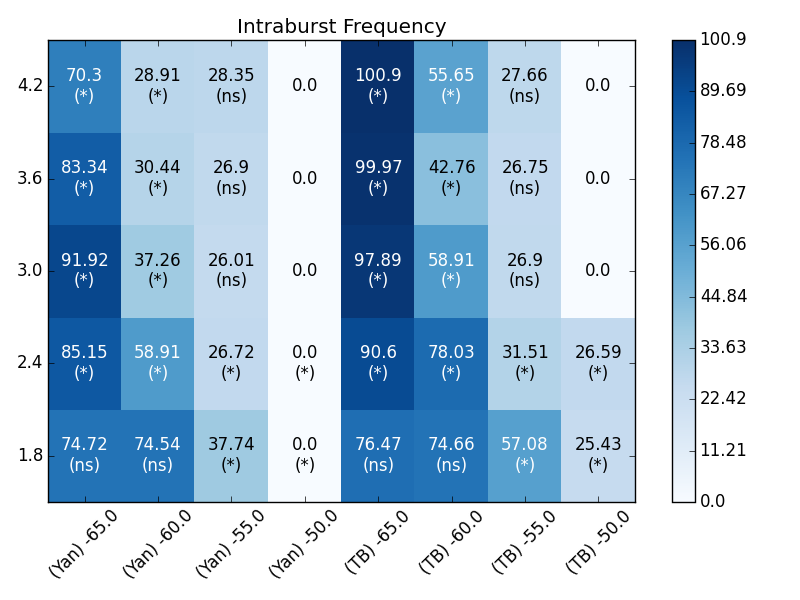
\includegraphics[scale=.4]{heatmap_Intraburst_Frequency.png}}%
	\subcaptionbox{Peaks per Burst \label{fig:hmPpB}}{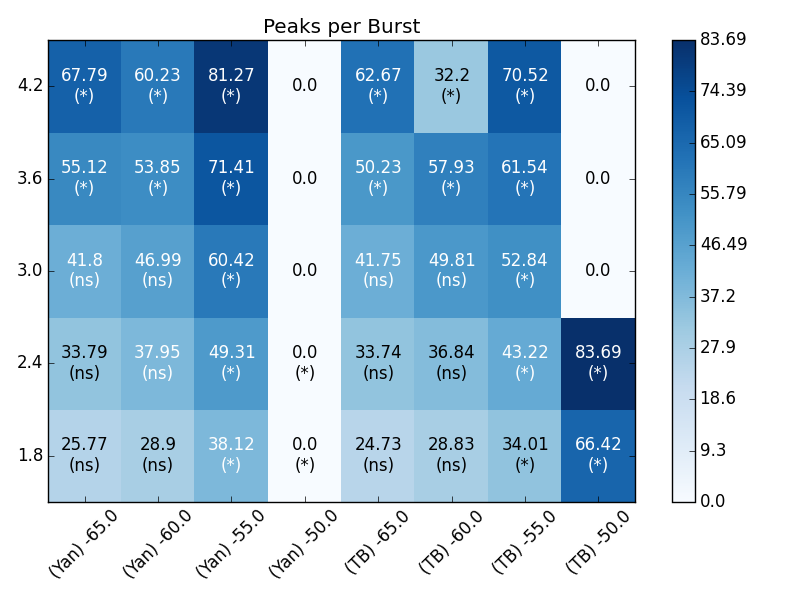
\includegraphics[scale=.4]{heatmap_Peaks_per_Burst.png}}%
	\caption{}
	\label{fig:hmPeakInBurst}
\end{figure}



\subsection{Peak Measures}
Average peak amplitude was showed strong model-dependent significant differences(Figure~\ref{fig:hmPA}). However, no clear and consistent pattern of increase or decrease occurred, making it difficult to tell if peak amplitude was model-dependent in a meaningful way. Interpeak interval (not pictured) was not model dependent, as no statistical significant difference occurred between same-parameters, different-model time series.
\begin{figure}[h]
	\centering
	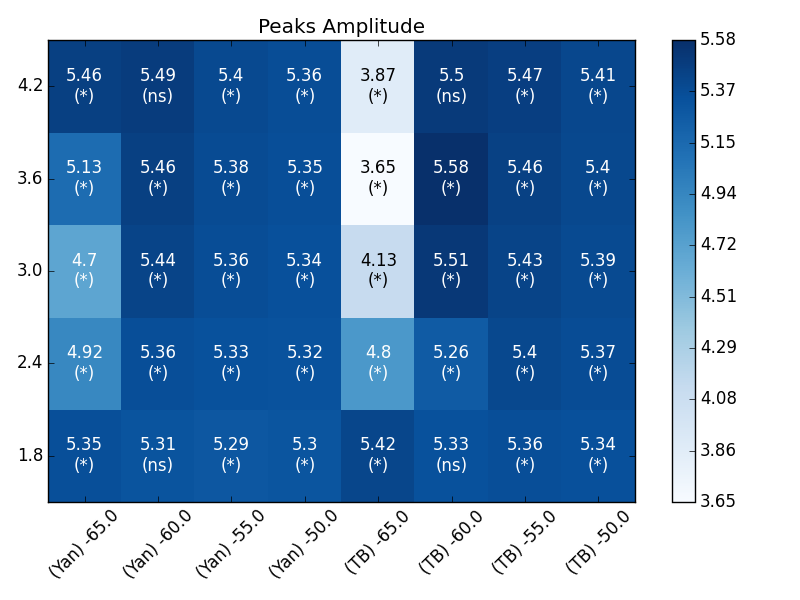
\includegraphics[scale=.4]{heatmap_Peaks_Amplitude.png}
	\caption{Peak Amplitudes. Stars (*) indicate  which cells were significantly different from their other-model counterpart.}
	\label{fig:hmPA}

\end{figure}



 
%\vspace{1.50cm}
%\noindent
\end{document}